\documentclass{article}
\usepackage{scribe}
\usepackage{amssymb}
\usepackage{amsmath}

\usepackage{csquotes}
\usepackage{amssymb}


\newtheorem{hw}{Homework Problem}
\newtheorem{ex}{Example}

\newcommand{\Perp}{{\bot\negthickspace\negthickspace\bot}}


%%% Unless you have very specific needs, the lines above should include
%%% all the typesetting features you need.

 


\begin{document}

\begin{lecture}{September 11th, 2019}{Lingfeng Zhang}{300134245}{lzhan278@uottawa.ca}

\section{Continue with Machine Learning Basis (Module 01)}

Continue with last lecture in Module 01. Start from Page 16 in the powerpoint

\textbf{Evaluation of a Learned Model}

Ultimate interest in out-of-sample performance(Testing dataset performance) versus in-sample(Training dataset performance)

\textbf{\textit{cross-validation}}

\begin{itemize}
\item Training dataset: to train the model

\item Validation dataset: to select hyper-parameters, to stop iterations, to check the performance of model

\item Testing dataset: to evaluate model performance
\end{itemize}

But sometimes we do not use validation set

\textbf{Fitting and Generalization}

Model too simple(like degree 1 polynomial): underfitting, shown in Figure \ref{fig:degree1polynomial}

\begin{figure}[ht!]
\centering
\scalebox{1}{
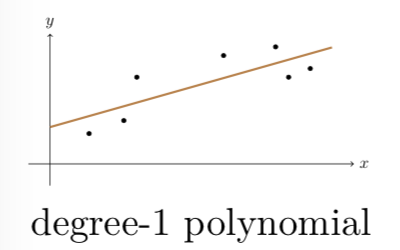
\includegraphics{images/degree1polynomial.png}}
\caption{degree-1 polynomial}
\label{fig:degree1polynomial}
\end{figure}


Model too complex(like degree large enough n polynomial): overfitting, shown in Figure \ref{fig:degree5polynomial}


\begin{figure}[ht!]
\centering
\scalebox{1}{
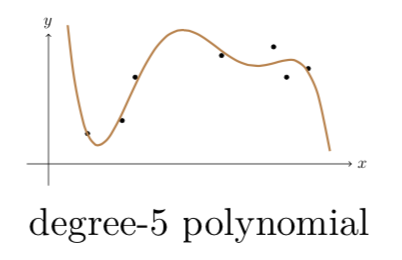
\includegraphics{images/degree5polynomial.png}}
\caption{degree-5 polynomial}
\label{fig:degree5polynomial}
\end{figure}


trade-off between simple model and complex model, shown in Figure \ref{fig:degree2polynomial}

\begin{figure}[ht!]
\centering
\scalebox{1}{
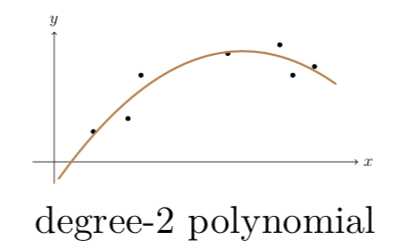
\includegraphics{images/degree2polynomial.png}}
\caption{degree-2 polynomial}
\label{fig:degree2polynomial}
\end{figure}

\begin{itemize}
\item In-Sample Error(training error): $E_{in}$
\item Out-of-Sample Error(testing error): $E_{out}$
\item Generalization Gap $E_{gen}:=E_{out},E_{in}$
\end{itemize}

The ideal situation: $E_{in}\approx 0$ and $E_{out}\approx E_{in}$

As shown in Figure \ref{fig:modelComplexityE}. When the model becomes more complex, $E_{in}$ decreases, $E_{out}$ decreases and then increases because the model from underfitting to fit well and then to overfitting,  $E_{gen}$ increases. The complexity bound between underfitting model and overfitting model reaches best model in this case.

\begin{figure}[ht!]
\centering
\scalebox{0.7}{
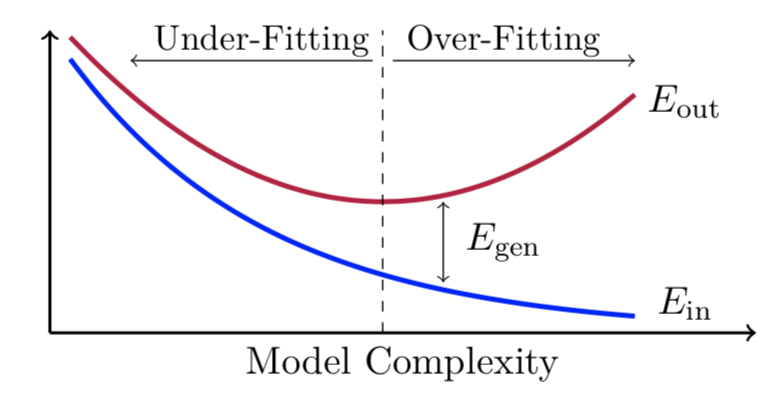
\includegraphics{images/modelComplexityE.png}}
\caption{E with different model complexity}
\label{fig:modelComplexityE}
\end{figure}

\textbf{Bias and Variance}

Mean square error is chosen as \emph{performance metric}

\textbf{\emph{Mathematical expectation}} is the summation or integration of a possible values from a random variable.

\begin{eqnarray}
E_{out} = \mathbb{E} _\mathcal{D} \mathbb{E} _\mathcal{X}(\hat f^{(\mathcal{D})}(X) - F(X))^2
\end{eqnarray}

In this case. We can look the equation(1) as two dimension mathematical expectation. one for Y-axis dimension(because there are maybe many y with respect to same x), another for the X-axis dimension(like common used expected value). The expectation $\mathbb{E} _\mathcal{D}$ can be understood as the integration of a possible error from a dataset with same x. The expectation $\mathbb{E} _\mathcal{X}$ can be understood as the integration of a possible error from the dataset with different x. See Figure \ref{fig:regressionPlot}. This also illustrate why $\mathbb{E} _\mathcal{D}\mathbb{E} _\mathcal{X}$ can be changed with $\mathbb{E} _\mathcal{X}\mathbb{E} _\mathcal{D}$

\begin{figure}[ht!]
\centering
\scalebox{1}{
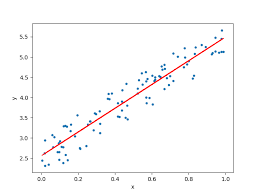
\includegraphics{images/regressionPlot.png}}
\caption{Regression Plot}
\label{fig:regressionPlot}
\end{figure}

\begin{eqnarray}
\bar f(x) := \mathbb{E} _\mathcal{D}\hat f^{(\mathcal{D})}(x)
\end{eqnarray}

$E_{out}$ decomposes into "bias" and "variance"

\begin{align*}
E_{out} &= \mathbb{E} _\mathcal{D} \mathbb{E} _\mathcal{X}(\hat f^{(\mathcal{D})}(X) - F(X))^2 \\
&= \mathbb{E} _\mathcal{X} \mathbb{E} _\mathcal{D}(\hat f^{(\mathcal{D})}(X) - F(X))^2 \\
&= \mathbb{E} _\mathcal{X} \mathbb{E} _\mathcal{D}(\hat f^{(\mathcal{D})}(X) - \bar f(X) +\bar f(X) - F(X))^2 \\
&= \mathbb{E} _\mathcal{X} \mathbb{E} _\mathcal{D} [ (\hat f^{(\mathcal{D})}(X) - \bar f(X))^2 +(\bar f(X) - F(X))^2 +\\ & \>\>\>\>\> 2(\hat f^{(\mathcal{D})}(X) - \bar f(X))(\bar f(X) - F(X))^2) ] \\
&= \mathbb{E} _\mathcal{X} \mathbb{E} _\mathcal{D}(\hat f^{(\mathcal{D})}(X) - \bar f(X))^2 +  \mathbb{E} _\mathcal{X} \mathbb{E} _\mathcal{D}(\bar f(X) - F(X))^2 + \\ & \>\>\>\>\> \mathbb{E} _\mathcal{X} \mathbb{E} _\mathcal{D}2(\hat f^{(\mathcal{D})}(X) - \bar f(X))(\bar f(X) - F(X))^2) \\
&= \mathbb{E} _\mathcal{X} \mathbb{E} _\mathcal{D}(\hat f^{(\mathcal{D})}(X) - \bar f(X))^2 +  \mathbb{E} _\mathcal{X} \mathbb{E} _\mathcal{D}(\bar f(X) - F(X))^2 \\
&= \mathbb{E} _\mathcal{X} \mathbb{E} _\mathcal{D}(\hat f^{(\mathcal{D})}(X) - \bar f(X))^2 +  \mathbb{E} _\mathcal{X} (\bar f(X) - F(X))^2 \\
:&= variance + bias 
\end{align*}

In process from step 3 to step 4. Look $\hat f^{(\mathcal{D})}(X) - \bar f(X)$ as a unit, and $\bar f(X) - F(X))^2$ as a unit

In process from step 5 to step 6. Due to the equation(2), $\mathbb{E} _\mathcal{X} \mathbb{E} _\mathcal{D}2(\hat f^{(\mathcal{D})}(X) - \bar f(X))(\bar f(X) - F(X))^2)$ is 0

In process from step 6 to step 7.$\mathbb{E} _\mathcal{D}$ is useless for $(\bar f(X) - F(X))^2$

As shown in Figure \ref{fig:biasVarianceTradeoff}. Grey circle represents high complexity model,green circle represents low complexity model, blue dot means $\bar f$, red dot means $\hat f^{(\mathcal{D})}$, F means true value ground.

\begin{itemize}
\item “Bias”: the error of $\bar f$ relative to the ground truth $F$ 

\item “Variance”: the average deviation of $\hat f^{(\mathcal{D})}$ relative to $\bar f$
\end{itemize}

The inability for a machine learning method to capture the true relationship is call bias.

In Machine Learning lingo, the difference in fits between data sets is called Variance.

Visiting \texttt{https://www.youtube.com/watch?v=EuBBz3bI-aA} to visualize these two lingo

Best situation: low bias, low variance

\begin{itemize}
\item Low complexity model: high bias(blue dot far away from F), low variance(red dot close to blue dot)

\item High complexity model: low bias(blue dot close F), high variance(red dot sparse around blue dot)
\end{itemize}

In polynomial regression problem, low complexity model is the subset of high complexity model.

\begin{figure}[ht!]
\centering
\scalebox{0.5}{
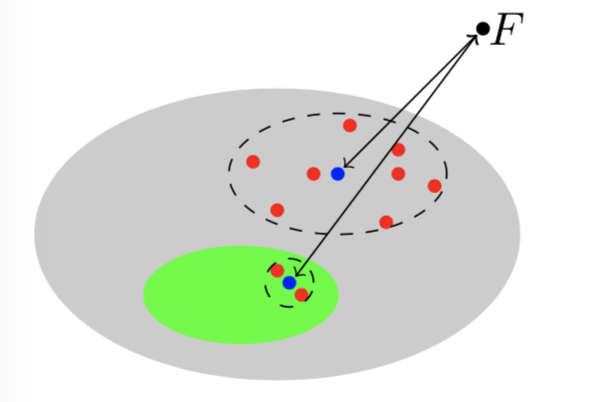
\includegraphics{images/biasVarianceTradeoff.png}}
\caption{bias vs. variance tradeoff}
\label{fig:biasVarianceTradeoff}
\end{figure}

\begin{figure}[ht!]
\centering
\scalebox{0.5}{
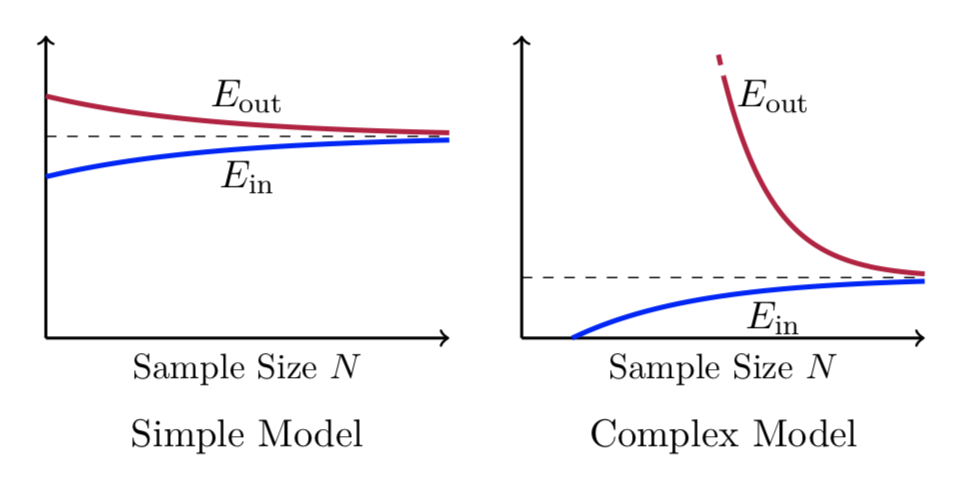
\includegraphics{images/sampleSizeE.png}}
\caption{E varies with sample size in different complexity model}
\label{fig:sampleSizeE}
\end{figure}

In classical theory, as shown in Figure \ref{fig:sampleSizeE}. Let us understand these plots by using the idea of mathematical limit. For the left plot(Simple Model plot), assuming I have 2 points as the training data, the simple model is the polynomial 2 model.This simple model can fit the 2-point training data well and its in-sample error is 0. About the out-sample, assuming testing sample size is 1000, the out-sample error will be extremely high because it is underfitting. With the increasing sample size,polynomial 2 model can not fit all training data well, so its in-sample error will increase, but the out-sample error will decrease because the model fits the larger training dataset better.If the sample size is large enough, in-sample error and out-sample error will be approximately equal. I guess this is because the noise will disappear in extremely large dataset. In left plot, the powerpoint captures the part of whole plot. The whole plot is shown in Figure \ref{fig:wholeSampleSizeE}. Simple model can not fit all training data well. So both in-sample error and out-sample error are high. For complex model, assuming I have 10 points as the training data, the simple model is the polynomial 20 model. If the sample size less than 10 points(sample size threshold) in this complex model, the in-sample error will always 0.Assuming the testing dataset size is 1000, the out-sample error will be extremely high, higher than simple model because it is overfitting too much.When the sample size increase, the in-sample error will increase and the out-sample error will decrease,finally they are converged. Complex model final error is lower than simple model because complex model can fit data better in large enough dataset.In general, the out-sample error is higher than in-sample error.

\begin{figure}[ht!]
\centering
\scalebox{0.5}{
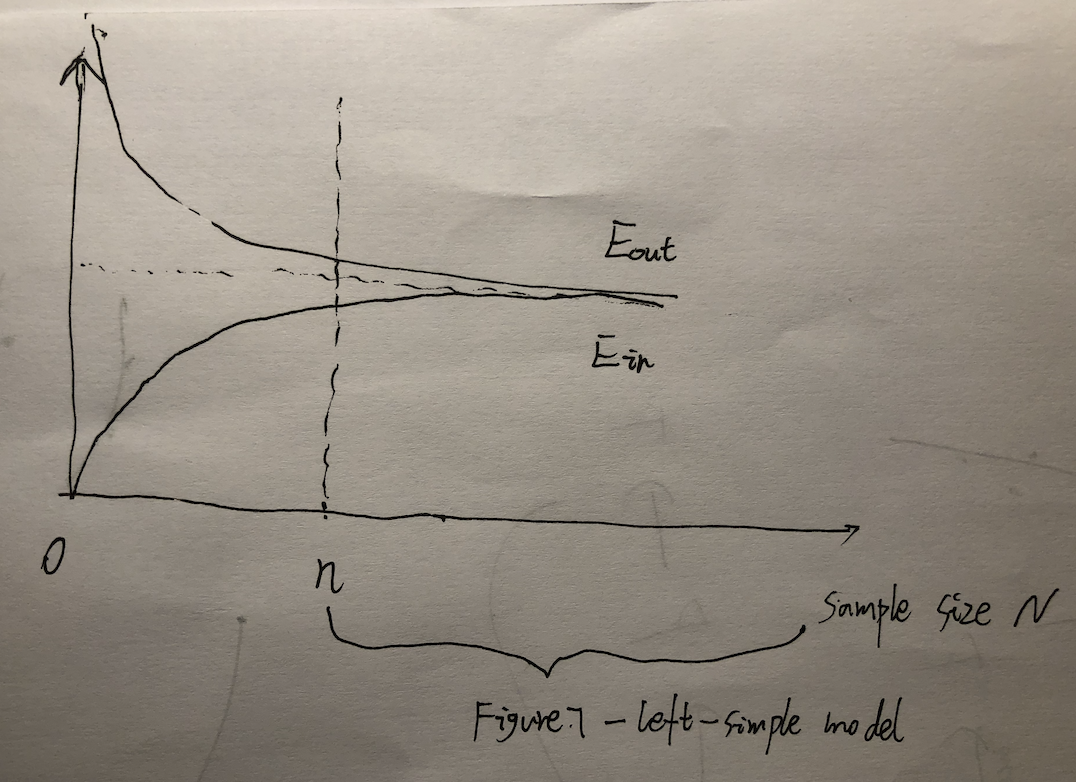
\includegraphics{images/wholeSampleSizeE.png}}
\caption{whole sample size N plot in simple model}
\label{fig:wholeSampleSizeE}
\end{figure}

In Figure \ref{fig:modernTheory}. It is the recent research about bias-variance tradeoff. When the model is complex enough, the test risk will decrease after its increasing.

\begin{figure}[ht!]
\centering
\scalebox{0.5}{
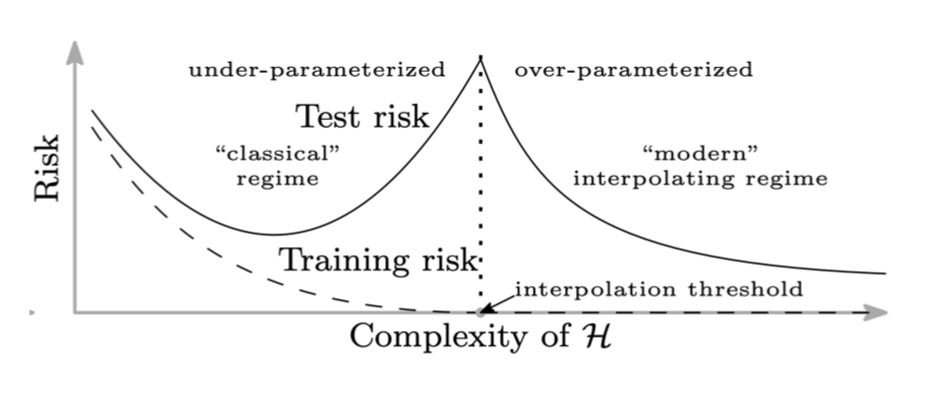
\includegraphics{images/modernTheory.png}}
\caption{recent theory of bias-variance tradeoff}
\label{fig:modernTheory}
\end{figure}

\begin{itemize}
\item Mikhail Belkin, Daniel Hsu, Siyuan Ma, Soumik Mandal,
Reconciling modern machine learning and the bias-variance trade-off
\item \texttt{https://arxiv.org/abs/1812.11118}
\item December 28,2018
\end{itemize}


\textbf{Regularization}

reduce overfitting in the complex model.

constrain parameter space to make smoother hypothesis(can stop early to realize)

\emph{regularized loss function}

\begin{eqnarray}
\mathcal{L}_{Reg}(\theta) := \mathcal{L}(\theta) + \Omega(\theta)
\end{eqnarray}

\textbf{L2-Regularizer}

a.k.a(as known as) "weight decay"

\begin{eqnarray}
\Omega(\theta) := \lambda_{Reg}\| \theta \| _2 ^2
\end{eqnarray}

$ \lambda_{Reg}$ is a hyper-parameter(decided parameter)

Larger $ \lambda_{Reg}$ makes $\| \theta \| _2$ smaller, because if $\| \theta \| _2$ is large with large $ \lambda_{Reg}$, the whole loss function will be large. $ \lambda_{Reg}$ acts as a judger to penalize large $\| \theta \| _2$.

\textbf{MAP Principle}

minimizing $\mathcal{L}(\theta) \Leftrightarrow$ ML formulation

minimizing $\mathcal{L}_{Reg}(\theta)$with L2-regularizer $ \Leftrightarrow$ maximum a posteriori (MAP) formulation with a Gaussian prior$p(\theta)$

Suppose that $\theta$ is drawn from a distribution $p_\theta$ on $\Theta$. The \textit{Maximum A Posteriori (MAP)} Principle estimate $\hat \theta_{MAP}$ of $\theta$ under a probability model is the value of $\theta$ that maximizes the $p(\theta|\mathcal{D})$:

\noindent \textit{Proof}:
        \begin{align*}
            \hat{\theta}_{MAP} :&= arg\max_{\theta}p (\theta|\mathcal{D})\\
            &= arg\max_{\theta}logp (\theta|\mathcal{D})\\
            &= arg\max_{\theta}log \frac{p (\theta |\mathcal{D})p(\theta )}{p(\mathcal{D})}\\
            &= arg\max_{\theta}log p (\theta |\mathcal{D})p(\theta )\\
            &= arg\max_{\theta}(log p (\theta |\mathcal{D})+logp(\theta ))\\
            &=arg\min_{\theta}(-log p (\mathcal{D}|\theta) - log p (\theta)) \\
            &=arg\min_{\theta}(\mathcal{L}(\theta) - log p (\theta)) 
        \end{align*}
        
In the progress from step 6 to 7. When $p (\mathcal{D})$ becomes maximum, $logp (\mathcal{D})$ becomes maximum(because logarithm function is increasable), $-logp (\mathcal{D})$ becomes minimum. It acts as minimizing the loss function(proved in last lecture).

$-log p(\theta)$ serves as a regularizer $\Omega(\theta)$. When $p(\theta)$ is a spherical Gaussian, $-log p(\theta)$ reduces to the weight-decay regularizer.

\textbf{Another View of Regularization}

\begin{align*}
minimizing \mathcal{L}_{Reg}(\theta) &\Leftrightarrow minimizing E_{out}\\
minimizing \mathcal{L}\theta) &\Leftrightarrow minimizing E_{in} \\
minimizing \Omega(\theta) &\Leftrightarrow minimizing E_{gen}
\end{align*}

$E_{gen}$ is small for simple model and large for complex model

$\Omega(\theta)$ is small for simple model and large for complex model

\textbf{Three key aspects of a Machine Learning model}

\begin{itemize}
    \item \textbf{Expressivity}: fit well in training data
    \item \textbf{Generalization}: generalize well from training data to testing data
    \item \textbf{Optimization}: effective and efficient mean to meet Expressivity and Generalization
\end{itemize}
    
\textbf{After class reading}

Deep Learning by Goodfellow, etc. Chapter 5

\section{Logistic and Soft-Max Regression(Module 02)}

\textbf{Binary Classification}

the target is binary {0,1}

classify the example X into corresponded classification

/textbf{Discriminative Modelling}

\begin{itemize}
\item modelling: conditional distribution hypotheses $p_{Y\mid X}$
\item learning:  find "best"(ML/MAP) distribution $\hat p_{Y\mid X}$
\item binary classification/prediction: 
	\begin{itemize}
	\item $\hat p_{Y\mid X}(1\mid x) > threshold value \Rightarrow$ first classification
	\item otherwise $\Rightarrow$ second classification
	\end{itemize}
\end{itemize}

\textbf{Maximizing likelihood = minimizing the cross entropy loss}

\begin{eqnarray}
CrossEntropy(\widetilde p; p) := - \sum_{y \in \mathcal{Y}} \tilde{p}(y) log p(y)
\end{eqnarray}

Assuming $(x_i,y_i)$'s are i.i.d

\noindent \textit{Proof}:
	\begin{align}
            \hat{p}_{Y|X}^{ML} :&= arg\max_{p_{Y|X} \in \mathcal{H}} p(\mathcal{D}|p_{Y|X}) \nonumber \nonumber \\ 
            &= arg\max_{p_{Y|X} \in \mathcal{H}} \prod_{i=1}^N p_{Y|X}(y_i\mid x_i) \nonumber \\
            &= arg\max_{p_{Y|X} \in \mathcal{H}} log \prod_{i=1}^N p_{Y|X}(y_i\mid x_i) \nonumber \\
            &= arg\min_{p_{Y|X} \in \mathcal{H}} \sum_{i=1}^N -log  p_{Y|X}(y_i\mid x_i) \nonumber \\
            &= arg\min_{p_{Y|X} \in \mathcal{H}} \sum_{i=1}^N \{ -\mathbb{I} \{y_i=1\} log_{p_{Y|X}} (1|x_i) - \mathbb{I} \{y_i = 0\} log_{p_{Y|X}} (0|x_i) \} \nonumber \\
            &= arg\min_{p_{Y|X} \in \mathcal{H}} \sum_{i=1}^N CrossEntropy \big( \mathbb{I} \{y_i = \cdot\} ; p_{Y|X}(\cdot|x_i) \big) \nonumber
        \end{align}

Illustration: $\mathbb{I} \{y_i=1\}=1$ if $y_i=1$; $\mathbb{I} \{y_i=1\}=0$ if $y_i=$ others

\textbf{Logistic Regression Model}

Logistic function/sigmoid function

\begin{eqnarray}
\sigma(x) := \frac{1}{1+e ^{-x}}
\end{eqnarray}

\begin{figure}[ht!]
\centering
\scalebox{0.5}{
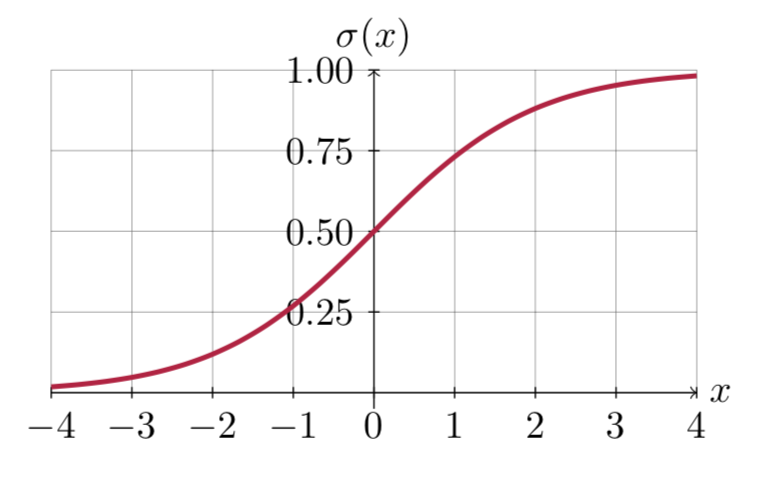
\includegraphics{images/sigmoid.png}}
\caption{Sigmoid function plot}
\label{fig:sigmoid}
\end{figure}

derivative property: $\sigma'(x) = \sigma(x)(1-\sigma(x))$

\noindent \textit{proof}:

\begin{align*}
\sigma'(x) &= \frac{e ^{-x}}{(1+e ^{-x})^2}\\
&= \frac{e ^{-x}}{(1+e ^{-x})^2} \\
&= \frac{1 \times(1+e ^{-x}-1)}{(1+e ^{-x})^2} \\
&= \sigma(x)(1-\sigma(x))
\end{align*}

\textbf{Logistic regression model}

$p_{Y \mid X} \in \mathcal{H}$

\begin{align}
p_{Y \mid X}(1 \mid x) :&= \sigma(w^Tx+b) \\
p_{Y \mid X}(0 \mid x) :&=1- \sigma(w^Tx+b)
\end{align}

where $w \in \mathcal{R}^m$ and $b$ is a scalar

the dimension of hyperplane = the dimension of ambient space - 1 

See Figure \ref{fig:geometrySigmoid}.$\sigma(\theta^Tx)=\frac{1}{2}$ means $<\theta ,x> = 0$. This case approximately never happen. $< \theta ,x >$ larger than 0, means it will be classified 1. Otherwise, it will be classified 0.

linear transformation $\Rightarrow$ affine transformation

Commonly, writing $w^Tx+b$ as $w^Tx$.

\begin{figure}[ht!]
\centering
\scalebox{0.5}{
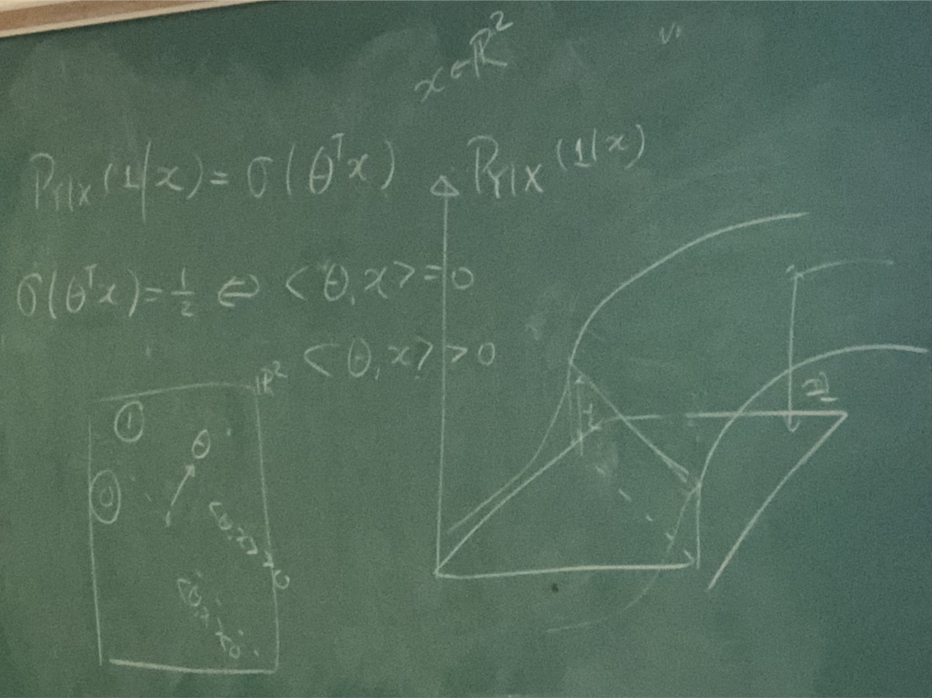
\includegraphics{images/geometrySigmoid.png}}
\caption{Geometry Illustration Sigmoid}
\label{fig:geometrySigmoid}
\end{figure}

Define loss $\mathcal{L}(w)$ by:

\begin{align}
\mathcal{L}(w) :&= \frac{1}{N} \sum_{i=1}^N CrossEntropy(\mathbb{I}{y_i=\cdot};p_{Y\mid X}(\cdot \mid x_i)) \\
&= \frac{1}{N} \sum_{i=1}^N \{y_i log \sigma(w^T x_i)+(1-y_i) log (1-\sigma(w^Tx_i))\} \nonumber
\end{align}

Progress from step 1 to step 2:  Reference equation (5), (7), (8)

To find $\hat w := atg\min_w \mathcal{L}(w)$

\begin{align}
\frac{d\mathcal{L}}{dw} &= -\frac{1}{N}\sum_{i=1}^Nx_i(y_i-\sigma(w^Tx_i))
\end{align}

When you calculate the $\frac{d\mathcal{L}}{dw}$, you can use $\sigma'(x) = \sigma(x)(1-\sigma(x))$

$\frac{d\mathcal{L}}{dw}$ can be applied to GD and Mini-Batched SGD

See Figure \ref{fig:logisticRegressionNN}. Logistic regression model can be represented as a simple neural network to classify binary-class data.

\begin{figure}[ht!]
\centering
\scalebox{0.5}{
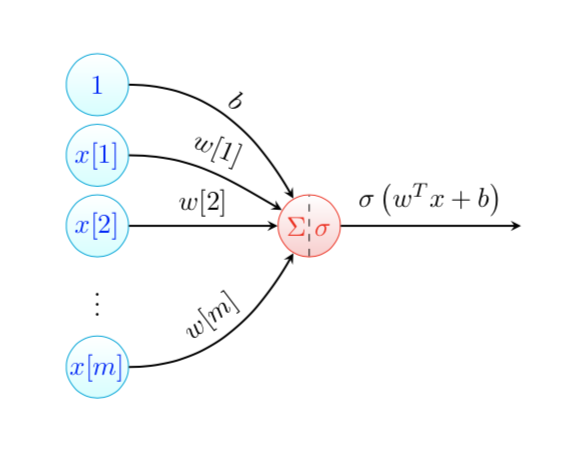
\includegraphics{images/logisticRegressionNN.png}}
\caption{Logistic Regression Model as a Simple Neural Network}
\label{fig:logisticRegressionNN}
\end{figure}

\textbf{Multi-Class Classification}

$\mathcal{Y}$ of labels contains $K$ elements.

Binary classification: $K=2$. 

Multi-Class classification: $K>2$. 
        
\textbf{Soft-max Function}

Converting the "scores" of $K$ objects into a probability distribution over the $K$ objects.

Larger score $\Rightarrow$ larger probability. 
            \[
                softmax: \mathbb{R}^K \rightarrow \mathbb{R}^K
            \]
            
For each $s \in \mathbb{R}$, $softmax(s)$ is the vector $q \in \mathbb{R}^K$ such that:

For each $i=1,2,\dots,K$

\begin{eqnarray}
q[i] = \frac{e^{s[i]}}{\sum_{j=1}^K e^{s[j]}}
\end{eqnarray}

When $K=2$  and $q:softmax(s)$

\begin{align*}
q[1] &=  \frac{e^{s[1]}}{\sum_{j=1}^2 e^{s[j]}} \\ 
&=  \frac{e^{s[1]}}{ e^{s[1]} + e^{s[2]}} \\ 
&= \frac{1}{1+\frac{e^{s[2]}}{e^{s[1]}}} \\
&= \frac{1}{1+e^{s[2]-s[1]}} \\
&= \frac{1}{1+e^{-(s[1]-s[2])}} \\
&= \sigma(s[1]-s[2])
\end{align*}

So, the soft-max function is a generalization of the logistic function.

\textbf{Jacobian of the soft-max function}

\noindent Lemma

Suppose that $s \in \mathcal(R)^K$ and $q=softmax(s)$. Then for any $i,j \in \{ 1,2, \dot, K \} $,

\begin{eqnarray*}
\frac{\partial q[i]}{\partial s[j]} = q[i](\delta_{ij} - q[j]) \\
\end{eqnarray*}

where $\delta_{ij} := \mathbb{I}\{i=j\}$

\noindent \textit{proof}:

When $i \neq j$

\begin{align*}
\frac{\partial q[i]}{\partial s[j]} &= - \frac{e^{s[i]}e^{s[j]}}{(\sum_{j=1}^K e^{s[j]})^2} \\
&= - \frac{e^{s[i]}}{\sum_{j=1}^K e^{s[j]}} \frac{e^{s[j]}}{\sum_{j=1}^K e^{s[j]}} \\
&= -q[i]q[j]
\end{align*}

When $i=j$

\begin{align*}
\frac{\partial q[i]}{\partial s[j]} &= \frac{\partial q[i]}{\partial s[i]} \\
&= \frac{e^{s[i]}\sum_{j=1}^K e^{s[j]}-{e^{s[j]}}^2}{(\sum_{j=1}^K e^{s[j]})^2} \\
&= \frac{e^{s[i]} (\sum_{j=1}^K e^{s[j]}-e^{s[j]})}{(\sum_{j=1}^K e^{s[j]})^2} \\
&= \frac{e^{s[i]} (\sum_{j=1}^K e^{s[j]}-e^{s[j]})}{(\sum_{j=1}^K e^{s[j]})^2} \\
&= \frac{e^{s[i]}}{\sum_{j=1}^K e^{s[j]}} \left( 1-\frac{e^{s[i]}}{\sum_{j=1}^K e^{s[j]}} \right) \\
&= q[i](1-q[i]) \\
&= q[i](1-q[j])
\end{align*}

\textbf{Properties of the soft-max function}
            \begin{itemize}
                \item For any scalar $c$, $softmax(s+c)=softmax(s)$
                \item Let $c$ be a positive scalar
                \begin{itemize}
                    \item If $c>1$, then $softmax(c \cdot s)$ has a higher ''contrast'' (i.e. peakier) than $softmax(s)$.  If $softmax(s[i]) > softmax(s[i])$,  then $softmax(c \dot s[i])$ becomes more larger than $softmax(c \dot s[j])$.
                    \item If $c<1$, then $softmax(c \cdot s)$ has a lower ''contrast'' (i.e. more uniform) than $softmax(s)$.  If $softmax(s[i]) > softmax(s[i])$,  then $softmax(c \cdot s[i])$ becomes less larger than $softmax(c \cdot s[j])$.
                \end{itemize}
            \end{itemize}
            
"contrast" means the variance of "scores"


            \textbf{Soft-max regression model}:
            \[
                p_{Y|X}(\cdot \mid  x) := softmax(Wx)
            \]
            where $W$ is a $K \times (m+1)$ matrix. Recall $x$ is a $(m+1)$ vector (after ``1'' is appended).

            \textbf{Soft-max regression learning}: find $\hat{W}$ that minimizes the cross-entropy loss (by GD or SGD).
            \[
                \mathcal{L}(W) := - \frac{1}{N} \sum_{i=1}^N log p_{Y|X} (y_i|x_i)
            \]

\textbf{Softmax Classification}: For each $x$, declare $arg\max_{y \in \mathcal{Y}} \hat{p}_{Y|X} (y|x)$ as its label.

See Figure \ref{fig:softmaxNN}. Softmax regression model can be represented as a simple neural network to classify multi-class data.

\begin{figure}[ht!]
\centering
\scalebox{0.5}{
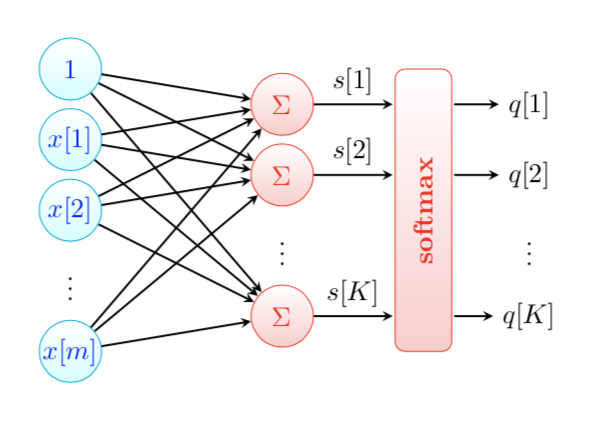
\includegraphics{images/softmaxNN.png}}
\caption{Softmax Regression Model as a Simple Neural Network}
\label{fig:softmaxNN}
\end{figure}


\end{lecture}

\end{document}
